\documentclass[10pt,twocolumn,letterpaper]{article}

\usepackage{cvpr}
\usepackage{times}
\usepackage{epsfig}
\usepackage{graphicx}
\usepackage{amsmath}
\usepackage{amssymb}
\usepackage{subcaption}
\usepackage{float}
\usepackage[style=ieee]{biblatex}

\addbibresource{biblio.bib}


\cvprfinalcopy % *** Uncomment this line for the final submission

\def\cvprPaperID{****} % *** Enter the CVPR Paper ID here
\def\httilde{\mbox{\tt\raisebox{-.5ex}{\symbol{126}}}}

\ifcvprfinal\pagestyle{empty}\fi
\begin{document}

\title{
Given Stereo Views Use 3D Reconstruction Algorithms to Reconstruct Terrain Topography \\
}


\author{Paul Borne--Pons, Quentin Gopée}
\maketitle

\section{Abstract}
The reconstruction of a 3D map from one or more images is a difficult problem still being researched today. In this project, we present a full pipeline to create this 3D map (disparity map) from stereo pairs of images. We first test our algorithms on middleburry \cite{VisionMiddleburyEdu} before using them to perform terrain reconstruction on extra terrestrial exploration images from NASA\cite{beyerAmesStereoPipeline2018}.

\section{Introduction}
The reconstruction of terrain topography using stereo image pairs and 3D reconstruction algorithms has garnered significant interest due to its potential applications in various fields like cartography, remote sensing, urban planning, and environmental monitoring. While this task can also be conducted by agents on the ground in some cases, there also exist senarios in which remote sensing is our only reliable way of measuring the topography not to mention that is in any case the most efficient way to retrive the topography of large areas. For example in the example of extra terrestrial exploration (the moon / moon / cassini mission) remote sensing satellite can acquire maps a land rover would much more difficulty be able to acquire. This study presents an basic explanation of a simple (yet complete) stereo vision pipeline and applications on the middleburry\cite{VisionMiddleburyEdu} dataset and setero pairs from NASA database of extra terrestrial exploration \cite{beyerAmesStereoPipeline2018}. In section 2 we will present the problem we are trying to solve and the related work. In section 3 we will present the methodology we used to solve the problem using SIFT\cite{lindebergScaleInvariantFeature2012} \& RANSAC\cite{fischlerRandomSampleConsensus1981} algorithms to perform epipolar rectification and graphcut algorithm for the density map estimation. In section 4 we will present the evaluation of our method on both middleburry and data from NASA and finally in section 5 we will conclude and discuss the results limitations of the proposed method.



\section{Problem Definition}

The problem we are trying to solve is the following: given a pair of stereo images, we want to compute the distance of each pixel to the camera (disparity map). This map is computed using the difference in the x coordinate of the same point in the two images between the two images of the stereo pair. In principle the procedure is quite straightforward but finding the pair of point for all pixel in the image is not an easy task as many problem can occur such as occlusion, noise, lighting not to mention the algorithmic complexity of the procedure. Furthermore, the disparity can only be computed (at least in a simple way) if the two images are have been taken from the same camera pose (same orientation but only a small translation between, the two camera centers) which call for rectification of the image pair before using the algorithm. 


\section{Related work}
Both the rectification and the disparity map estimation are well-known problems in computer vision. In this section, we discuss state-of-the-art methods for disparity map estimation from stereo images.


\subsection{Rectification of Stereo Pairs}

Stereo image rectification is an essential step in stereo vision pipelines. It aims to transform the stereo image pair such that the epipolar lines become horizontal and aligned. This transformation simplifies the disparity estimation process by reducing the search space to one dimension. Rectification is typically performed using the fundamental matrix computed from the stereo pair. Various algorithms, are used to compute the fundamental matrix and estimate the relative pose of the cameras. Once the fundamental matrix is obtained, the rectification transformation can be applied to the stereo pair to align the epipolar lines. This step ensures accurate and reliable disparity map estimation.

Several methods have been proposed for stereo image rectification, including geometric-based methods like SIFT\cite{lindebergScaleInvariantFeature2012}, RANSAC\cite{fischlerRandomSampleConsensus1981} and LMEDS \cite{lmeds} and deep learning-based methods like LIFT\cite{yiLIFTLearnedInvariant2016}, RANSAC-Flow \cite{shenRANSACFlowGenericTwostage2020}, Epipolar supervision \cite{darmonLearningGuideLocal2020}, Deep MVS\cite{huangDeepMVSLearningMultiview2018} and more recently NERFs\cite{mildenhallNeRFRepresentingScenes2020}. Geometric-based methods rely on geometric transformations and camera calibration parameters to rectify the stereo pair. Deep learning-based methods, on the other hand, leverage convolutional neural networks to learn the rectification transformation directly from the stereo images or to help compute one of the elements needed for the rectification (pixel pairs or F matrix). These methods have shown promising results in improving the accuracy and efficiency of stereo image rectification.

\subsection{Semi-Global Matching (SGM)}

Semi-Global Matching\cite{hirschmullerAccurateEfficientStereo2005a} (SGM) is a popular method for computing the disparity map. It takes advantage of the global information by aggregating the matching costs along multiple paths in a cost volume. SGM incorporates various penalties, such as uniqueness, smoothness, and occlusion, to improve the accuracy of the disparity map. It has been widely used in stereo matching applications due to its robustness and efficiency.

\subsection{Graph Cuts}

Graph cuts-based methods have also been extensively used for disparity map estimation \cite{kolomogorov}. These methods formulate the disparity estimation problem as an energy minimization problem, where the energy function is defined over a graph. By applying graph cuts, the disparity map is obtained by finding the minimum cut in the graph. Graph cuts-based methods have shown promising results in handling occlusions and preserving depth discontinuities.

\subsection{Deep Learning Approaches}

With the recent advancements in deep learning, convolutional neural networks "CNNs" \cite{schmidhuberDeepLearningNeural2015} have been applied to stereo matching tasks. These methods learn the mapping between stereo image pairs and their corresponding disparity maps using large-scale training datasets. Deep learning approaches have achieved state-of-the-art performance in disparity map estimation, surpassing traditional methods in terms of accuracy and robustness.

\subsection{Local  Methods}

Local methods for disparity map estimation focus on matching small image patches between the left and right images. These methods typically use similarity measures, such as sum of absolute differences (SAD) or normalized cross-correlation (NCC), to find the best matching patch. Local methods are computationally efficient but may struggle with handling occlusions and textureless regions.

These are just a few examples of the many methods available for disparity map estimation from stereo images. Each method has its own strengths and limitations, and the choice of method depends on the specific requirements of the application.


\section{Methodology}
The method chosen for this project isn't the most recent or the most accurate but it is a good compromise between accuracy and simplicity of implementation. The method is based on the following steps:
\subsection{Image rectification}

The image rectification pipeline is the following, we first use the SIFT algorithm to get the matching point between the two images of the stereo pair. Then using the matches we compute the fundamental matrix to get a better understanding of the relative pose of the two cameras. This matrix is usefull to compute the epipolar rectification. This step is needed as the transformation from a camera pose to another might be more complex than a translation (and a simple translation along one axis simplifies the search for the disparity as we only need to look for the disparity along one axis). Finally we use a graphcut \cite{kolomogorov} algorithm to retrieve the disparity map. In the project we decided to use OpenCV implementation for the SIFT\cite{lindebergScaleInvariantFeature2012} and epipolar rectification procedure. In this project we use OpenCV implementation for SIFT and epipolar rectification.
\subsubsection{SIFT}
The SIFT \cite{lindebergScaleInvariantFeature2012} algorithm is used to find the matching points between the two images of the stereo pair. The algorithm is the following, we first detect the keypoints in the two images using the Difference of Gaussian (DoG) algorithm. Then we compute the descriptors for each keypoint using the gradient of the image. Finally we match the descriptors using the nearest neighbor algorithm. The matching points are then used to compute the fundamental matrix.


\textbf{Scale Space:} SIFT operates on multiple scales of an image to detect features regardless of their size. This is achieved by constructing a scale space using Gaussian blurring and difference-of-Gaussian (DoG) techniques. The scale space represents the image at different levels of blur, allowing features to be detected at various scales.

\textbf{Keypoint Detection:} SIFT identifies keypoints or interest points in an image by locating local maxima and minima in the DoG pyramid. These keypoints are positions in the image that are invariant to changes in scale and orientation.

\textbf{Orientation Assignment:} Once keypoints are detected, SIFT computes their orientations to make them invariant to image rotation. It analyzes local gradients around each keypoint to assign a dominant orientation, enabling the descriptor to be rotationally invariant.

\textbf{Descriptor Generation:} The SIFT descriptor is a representation of the local image gradient distribution around a keypoint. It's formed by dividing the region around the keypoint into smaller subregions, calculating gradient orientations, and creating a histogram of gradient magnitudes and orientations. This descriptor encapsulates information about the keypoint's appearance.


The core mathematical operations in SIFT involve convolutions with Gaussian kernels, computation of image gradients, and histogram generation for the descriptors.

The Gaussian function $G(x, y, \sigma)$ is central to SIFT and represents the scale space. It is defined as:
\[ G(x, y, \sigma) = \frac{1}{2\pi\sigma^2} e^{-\frac{x^2 + y^2}{2\sigma^2}} \]
where $x$ and $y$ are spatial coordinates, and $\sigma$ is the scale parameter controlling the amount of blur.

The DoG (Difference of Gaussian) pyramid is obtained by subtracting adjacent Gaussian-blurred images at different scales:
\[ D(x, y, \sigma) = (G(x, y, k\sigma) - G(x, y, \sigma)) \ast I(x, y) \]
where $I(x, y)$ is the original image and $k$ is a constant determining the scale factor between adjacent levels.

Gradient orientation and magnitude are calculated using derivative filters (such as Sobel filters) to determine the local image gradients required for orientation assignment and descriptor generation.

The SIFT descriptor involves dividing the local region around a keypoint into smaller subregions (e.g., a 16x16 window), computing gradient orientations, and constructing histograms of gradient magnitudes and orientations within these subregions.

These mathematical operations collectively enable SIFT to detect and describe robust features in images, allowing for robustness to scale, rotation, and illumination changes.

\subsubsection{Epipolar Geometry}
To understand Epipolar Geometry lets first look at a basic stereo vision setup given in image
\begin{figure}[ht]
    \centering
    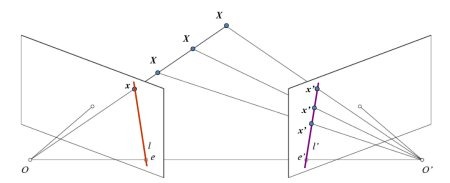
\includegraphics[width=0.4\textwidth]{epipolar.jpg}
    \caption{Stereo Vision Setup}
    \label{fig:stereo_vision_setup}
\end{figure}


Let's define:

\begin{itemize}
    \item \(O\) and \(O'\) as the camera centers.
    \item \(x\) as a point in the left image.
    \item \(x'\) as the corresponding point in the right image.
    \item \(e\) as the epipole in the left image.
    \item \(e'\) as the epipole in the right image.
\end{itemize}

The concept revolves around the Epipolar Geometry:

\begin{itemize}
    \item \textbf{Triangulation :} Using both left and right images allows for the triangulation of a 3D point corresponding to \(x\) by considering how different points on the line \(OX\) project onto different points \(x'\) in the right plane. This facilitates determining the correct 3D point.
    
    \item \textbf{Epipolar Constraint :} The projection of different points on \(OX\) forms a line (\(l'\)) on the right plane, known as the epiline corresponding to point \(x\). To find point \(x\) on the right image, searching along this epiline suffices. This constraint limits the search area to the epiline, enhancing performance and accuracy in finding matching points in the other image.
    
    \item \textbf{Epipolar Plane :} The plane \(XOO'\) is termed the Epipolar Plane, defining the relationship between the two cameras and their respective images.
    
    \item \textbf{Epipoles :} \(e\) and \(e'\) are the epipoles, where \(e\) is the point where the projection of the right camera \(O'\) is seen on the left image, and \(e'\) is similarly the point where the projection of the left camera \(O\) is seen on the right image. Sometimes, the epipoles might be located outside the image if one camera cannot see the other.
\end{itemize}

The relationship between epilines and epipoles:

\begin{itemize}
    \item All epilines pass through their respective epipoles.
    \item To locate the epipole, finding the intersection point of multiple epilines becomes a method to approximate its position.
\end{itemize}

The Epipolar Geometry is defined by the Fundamental Matrix \(F\), which is a \(3 \times 3\) matrix that relates corresponding points in the two images. It is defined as:

\[
x'^T \times F \times x = 0
\]

where \(x\) and \(x'\) are the corresponding points in the two images. The Fundamental Matrix is a rank 2 matrix, and it has 7 degrees of freedom. 

Fundamental Matrix F, maps a point in one image to a line (epiline) in the other image directly in the pixel coordinates without any need for camera calibration. The method used to compute the Fundamental Matrix from matches given by SIFT is described in the next section.


\subsubsection{RANSAC}
For each iteration of RANSAC\cite{fischlerRandomSampleConsensus1981}, we first sample 8 points from the matches.
We transform the points so  they are normalized
The normalizing factors are stored in the \(N\) matrix:

\[
N = \begin{bmatrix}
    \frac{1}{\bar{x}} & 0 & 0\\
    0 & \frac{1}{\bar{y}} & 0 \\
    0 & 0 & 1
\end{bmatrix}
\]

Then we compute the Fundamental matrix using the normalized points. The Fundamental matrix is computed using the SVD of the matrix \(A\). The \(A\) matrix is formed by stacking the points as follows:

\[
A = \begin{bmatrix}
    x_1x_1' & x_1y_1' & x_1 & y_1x_1' & y_1y_1' & y_1 & x_1' & y_1' & 1 \\
    x_2x_2' & x_2y_2' & x_2 & y_2x_2' & y_2y_2' & y_2 & x_2' & y_2' & 1 \\
    \vdots & \vdots & \vdots & \vdots & \vdots & \vdots & \vdots & \vdots & \vdots \\
    x_8x_8' & x_8y_8' & x_8 & y_8x_8' & y_8y_8' & y_8 & x_8' & y_8' & 1 \\
    0 & 0 & 0 & 0 & 0 & 0 & 0 & 0 & 0
\end{bmatrix}
\]

We have one row per point pair, and the last row of the \(A\) matrix is set to all 0 to ensure a square matrix for faster computation of SVD.

The Fundamental matrix is the last column of the \(V\) matrix of the SVD. The Fundamental matrix is then reshaped to a \(3 \times 3\) matrix, and then the SVD is applied again to the Fundamental matrix. The last singular value is set to 0, and the Fundamental matrix is recomputed using the formula \(F = USV^T\).

The Fundamental matrix is then denormalized using the \(N\) matrix and returned using the formula \(F = N^T \times F \times N\).

The Fundamental matrix is then returned, and the number of inliers is computed by counting the number of inliers that are at a distance less than 0.01 from the epipolar line. The distance is computed using the formula:

\[
d = \frac{|x' \times F^T \times x|}{\sqrt{(F^T \times x)_1^2 + (F^T \times x)_2^2}}
\]

where \(x'\) is the point in the second image and \(x\) is the point in the first image. We get a list of inliers, and the Fundamental matrix with the maximum number of inliers is returned.

We iterate over the RANSAC algorithm as long as the number of iterations is lower than:

\[
N_{\text{iter}} = \frac{\log(\text{threshold})}{\log(1 - \left(\frac{m}{n}\right)^8)}
\]

where \(m\) is the maximum number of inliers found so far and \(n\) is the total number of matches.

Finally, once all inliers are found, we compute the Fundamental matrix using all the inliers (we have a matrix \(A\) that is \(9 \times \text{num\_matches}\)) and compute the Fundamental matrix using the same method as before.

\subsubsection{Rectification from Fundamental Matrix}

Once the Fundamental matrix is computed, we can compute the rectification transformation. This transformation take the form of 2 homographies \(H_1\) and \(H_2\) used to transform the left and right images respectively. 

\begin{figure}[htbp]
    \centering
    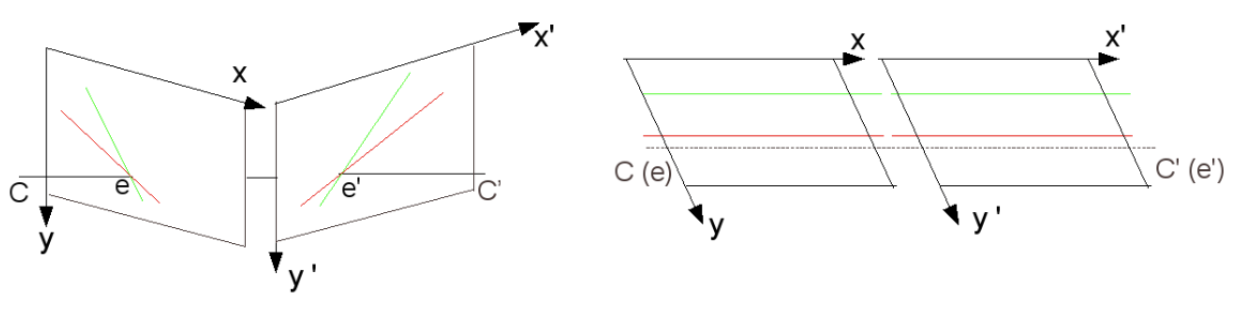
\includegraphics[width=0.5\textwidth]{rectification.png}
    \caption{Rectification illustration. Left: original cameras configuration. Right:
    Camera configuration after rectification. Image planes are coplanar and their
    x-axis is parallel to the baseline CC'}
    \label{fig:rectification}
\end{figure}

Note that the solution to the rectification is not unique. Once the rectifi-
cation is achieved, we can rotate two cameras together around the baseline
and the resulting images remain rectified. But the introduced projective
distortion is not different. The ideal is to achieve the rectification by
introducing a projective distortion as small as possible.




\subsubsection{Rectification from Essential Matrix}
\subsection{Disparity Map estimation}


We present a method to create a 3D disparity map utilizing graph cuts for increased robustness compared local methods. The approach employs the graph cut method to derive the disparity map.

Our disparity estimation involves multi-label optimization. Given two rectified images, we aim to assign the optimal disparity label \(l \in L\) to each pixel \(p \in P\). This problem translates to an energy minimization objective, where we seek a labeling \(f^* : P \rightarrow L\) that minimizes the energy \(E\), defined as:

\[
E(f) = \sum_{p \in P} D_p(f_p) + \sum_{(p,q) \in N} V_{p,q}(f_p,f_q)
\]

Here, \(D_p(f_p)\) represents the data term, \(V_{p,q}(f_p,f_q)\) denotes the smoothness term, and \(N\) signifies the set of neighboring pixel pairs within the image.

To minimize this energy function, we employ graph cuts, as demonstrated by the Kolmogorov and Zabih theorem in 2004 \cite{kolomogorov}. This theorem establishes the existence of a graph where the minimum cut corresponds to a labeling 'f' that achieves the minimum energy. To reformulate this problem as a graph cut problem, we create a graph structure explicitly representing the energy function we wish to minimize. The minimal \(f\) corresponding to the minimal cut yields the disparity map.
\begin{figure}[htbp]
    \centering
    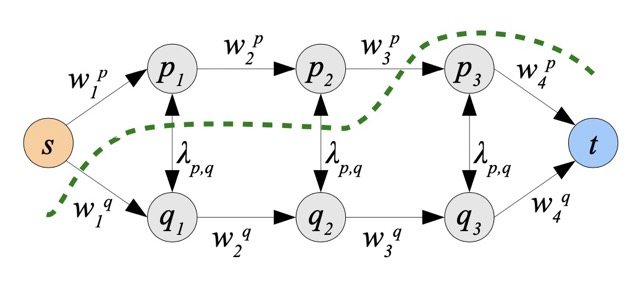
\includegraphics[width=0.4\textwidth]{graph.jpeg}
    \caption{Graph for Disparity Map Estimation}
    \label{fig:graph}
\end{figure}

\subsubsection{Linear Multi-label Graph Construction}

For our setup, \(L=\{ d_{\text{min}}, \dots, d_{\text{max}}\}\), with two rectified images of size \(512 \times 512\). The approach involves constructing one layer per disparity value and extracting the disparity value from the cut location.

\begin{itemize}
    \item The weights \(W_j^p\) represent the data term in \(E(f)\), computed using ZNCC (Zero-mean Normalized Cross-Correlation).
    \[
    D_p(j)=W_j^p=wcc \times \rho[E_{ZNCC}(P ; (j ,0))]
    \]
    Where:
    \[
    E_{ZNCC}(P;u) = \frac{1}{|P|} \sum_{q \in P} \left[\frac{(I'q + u - I'P)}{\sigma'} \cdot \frac{(Iq - IP)}{\sigma}\right]
    \]
    \[
    \rho(x) = \begin{cases}
        \frac{1}{1 + \exp(-x)}, & \text{if } x > 0 \\
        1, & \text{otherwise}
    \end{cases}
    \]
    Here, \(P\) represents a patch center in \(p\).
    
    \item To prevent multiple disparity cuts for the same pixel, we introduce a \(K_p\) penalty to the weights, assured by a lemma from Boykov et al. 1998:
    \[
    K_p = 1 + (k-1) \sum_{q \in N_p} \lambda_{p,q}
    \]
    \(K_p\) remains relatively consistent for each pixel, typically having between 2 and 4 neighbors. Consequently, we apply the penalization for 4 neighbors to all nodes.
    
    \item To accommodate the smoothness term in \(V\), we add edges between pixel neighbors along the same disparity dimension with the weight \(\lambda\).
\end{itemize}

\subsubsection{Patch-wise Implementation}

To optimize computation, we construct the graph not for each pixel but every 2 pixels. However, it's crucial to consider the central pixel of the patch in the image when computing the NCC. This approach also affects the indexing of nodes in the graph.


\section{Evaluation}
\subsection{Image rectification}
We propose an implementation of RANSAC tested on an easy pair of stereo images presented in Figure \ref{fig:stereo pair}. By stereo we mean a image pair where the two camera poses are quite similar which yields a lot of matches through the sift algorithm. We do not test on the middleburry dataset as the dataset is composed of stereo pairs that are already rectified. 


\begin{figure}
    \centering
    \begin{minipage}[t]{0.32\textwidth}
    \centerline{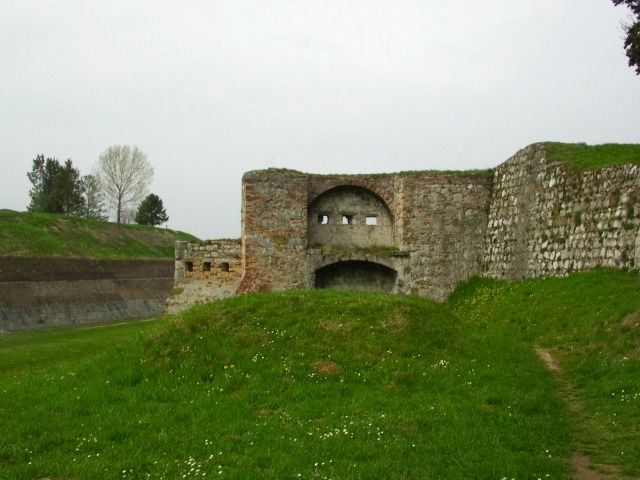
\includegraphics[width=\textwidth]{im1.jpg}}
    \centerline{Left Image}
    \end{minipage}
    \hfill
    \begin{minipage}[t]{0.32\textwidth}   
    \centerline{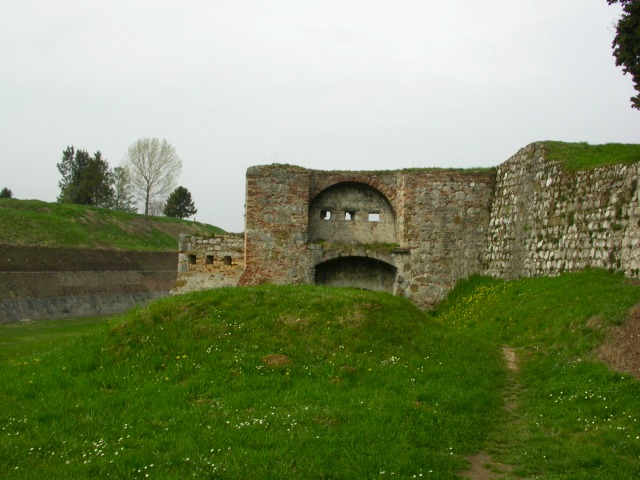
\includegraphics[width=\textwidth]{im2.jpg}}
    \centerline{Right Image}
    \end{minipage}
    \caption{Stereo pair of images}
    \label{fig:stereo pair}
\end{figure}

After running the SIFT algorithm on the two images we get the following matches and filtering the matches using the distance 
\begin{figure}
    \centering
    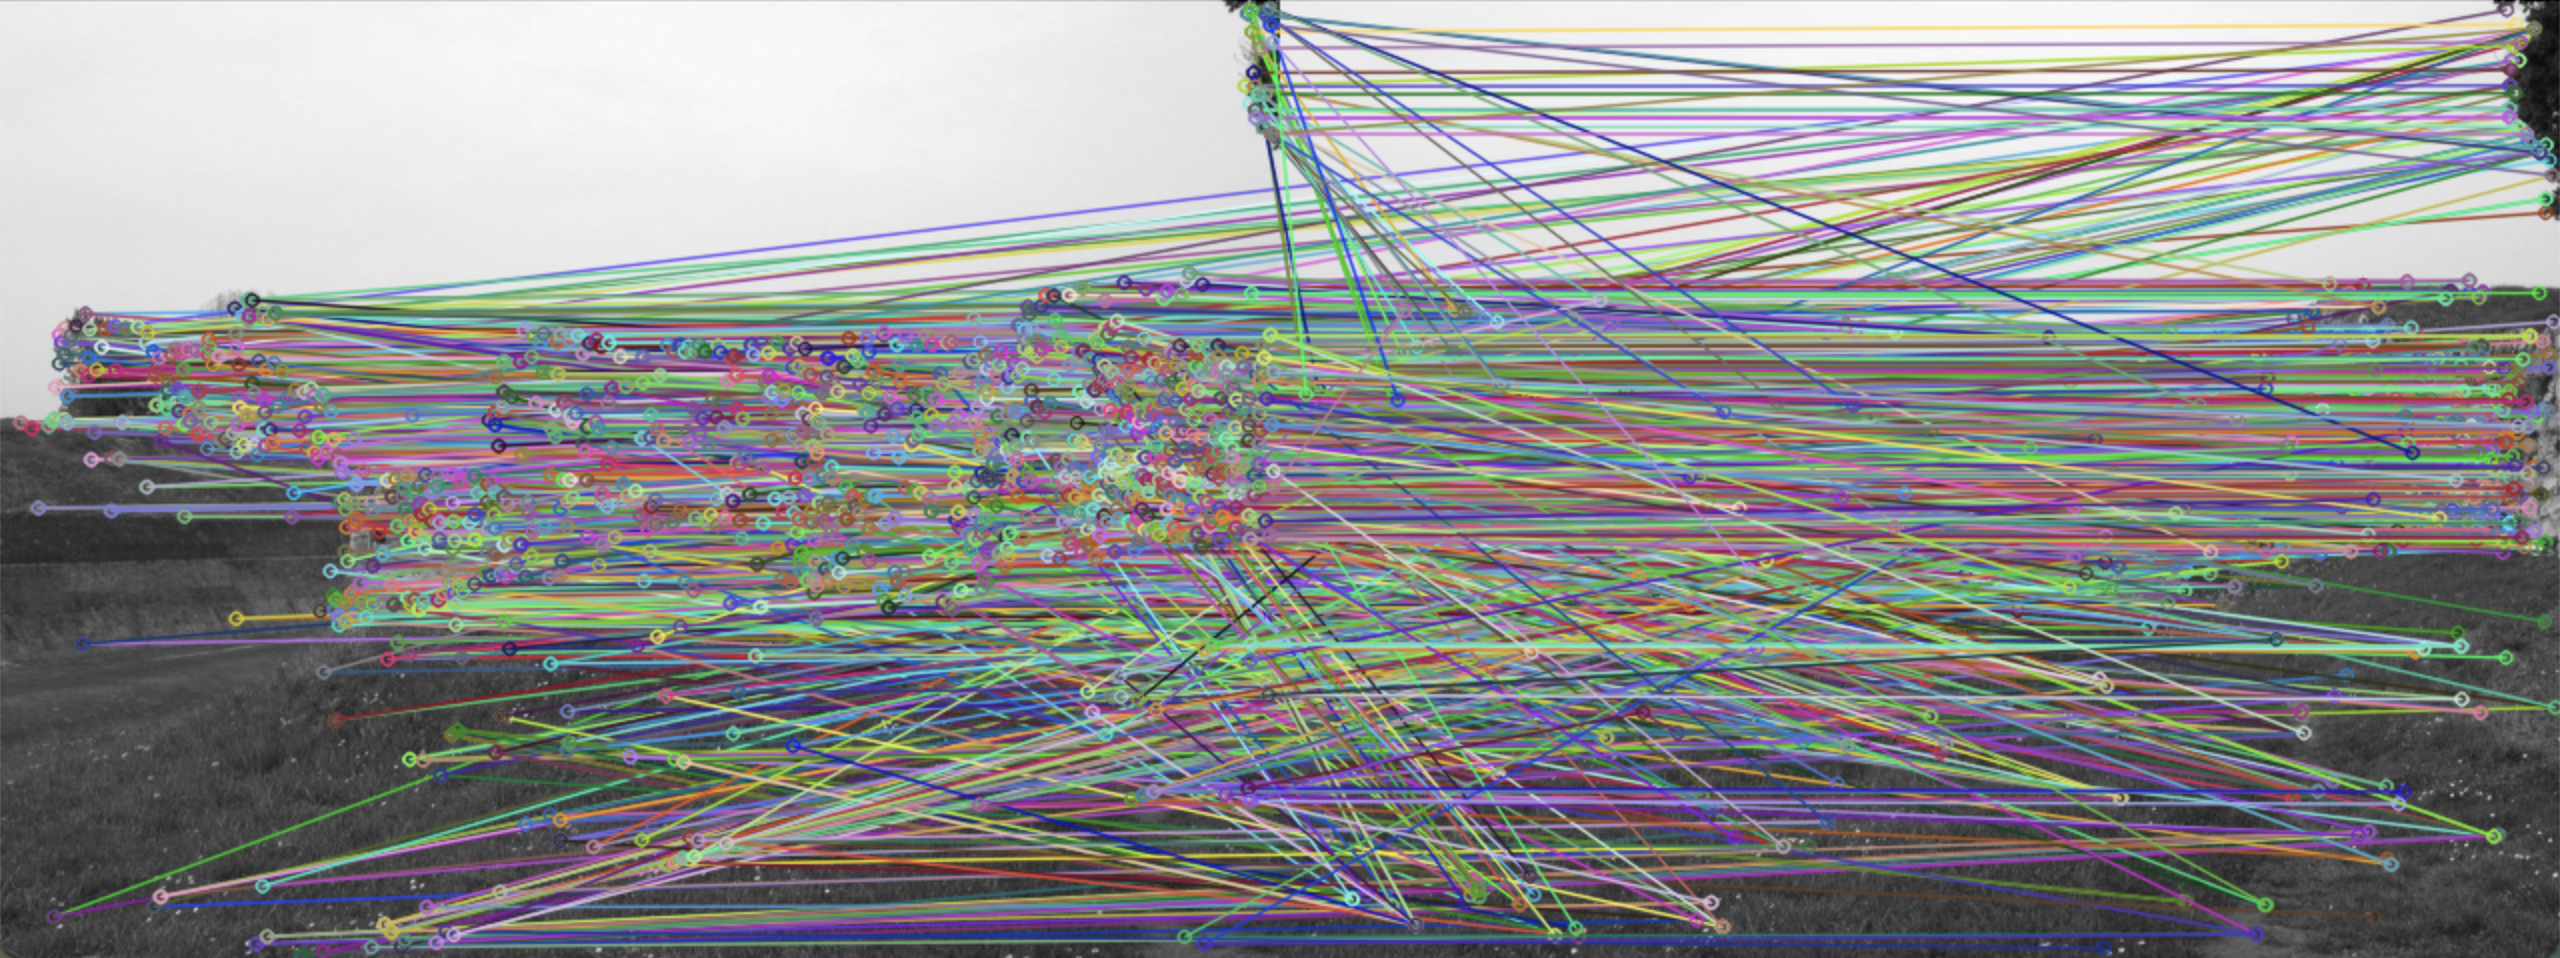
\includegraphics[width=0.5\textwidth]{sift.png}
    \caption{Matches between the two images}
    \label{fig:matches}
\end{figure}

We can see that a lot of these matches are not correct. We can see that the matches are not correct as they are not aligned on the same line.  To solve this problem we use the RANSAC algorithm to find the fundamental matrix which will jointly give us the F matrix and sort the inliers from the outliers.
As a result we get approximately 400 to 500 inliers (as the algorithm is stochastic the number of inliers varies from one run to another). We can see the result in figure \ref{fig:ransac}.
\begin{figure}
    \centering
    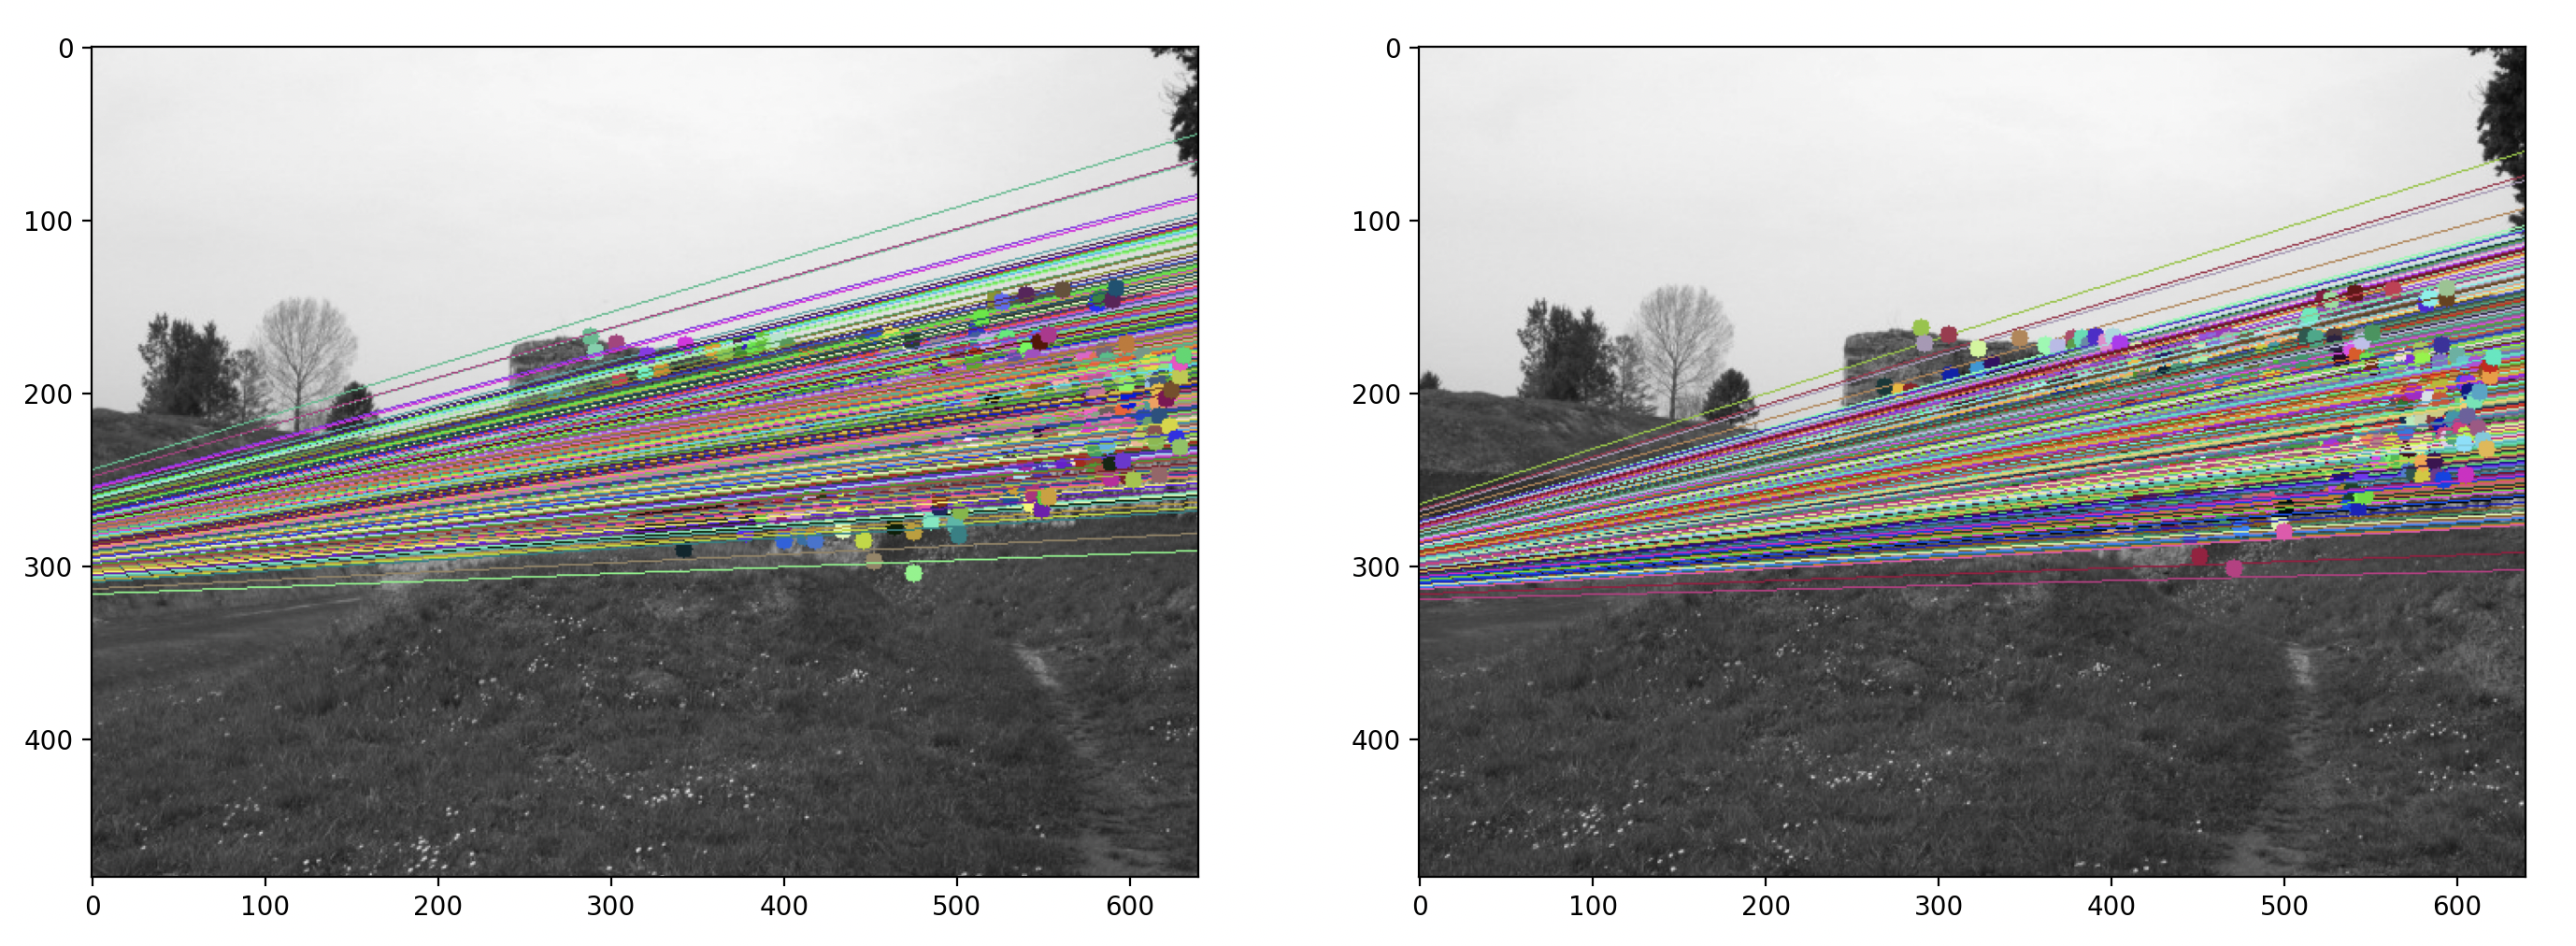
\includegraphics[width=0.5\textwidth]{easy_ransac.png}
    \caption{Matches between the two images after RANSAC}
    \label{fig:ransac}
\end{figure}

Using the learnt fundamental matrix we can now compute the epipolar rectification. The result is shown in figure \ref{fig:rectified stereo pair}.

\begin{figure}
    \centering
    \begin{minipage}[t]{0.32\textwidth}
    \centerline{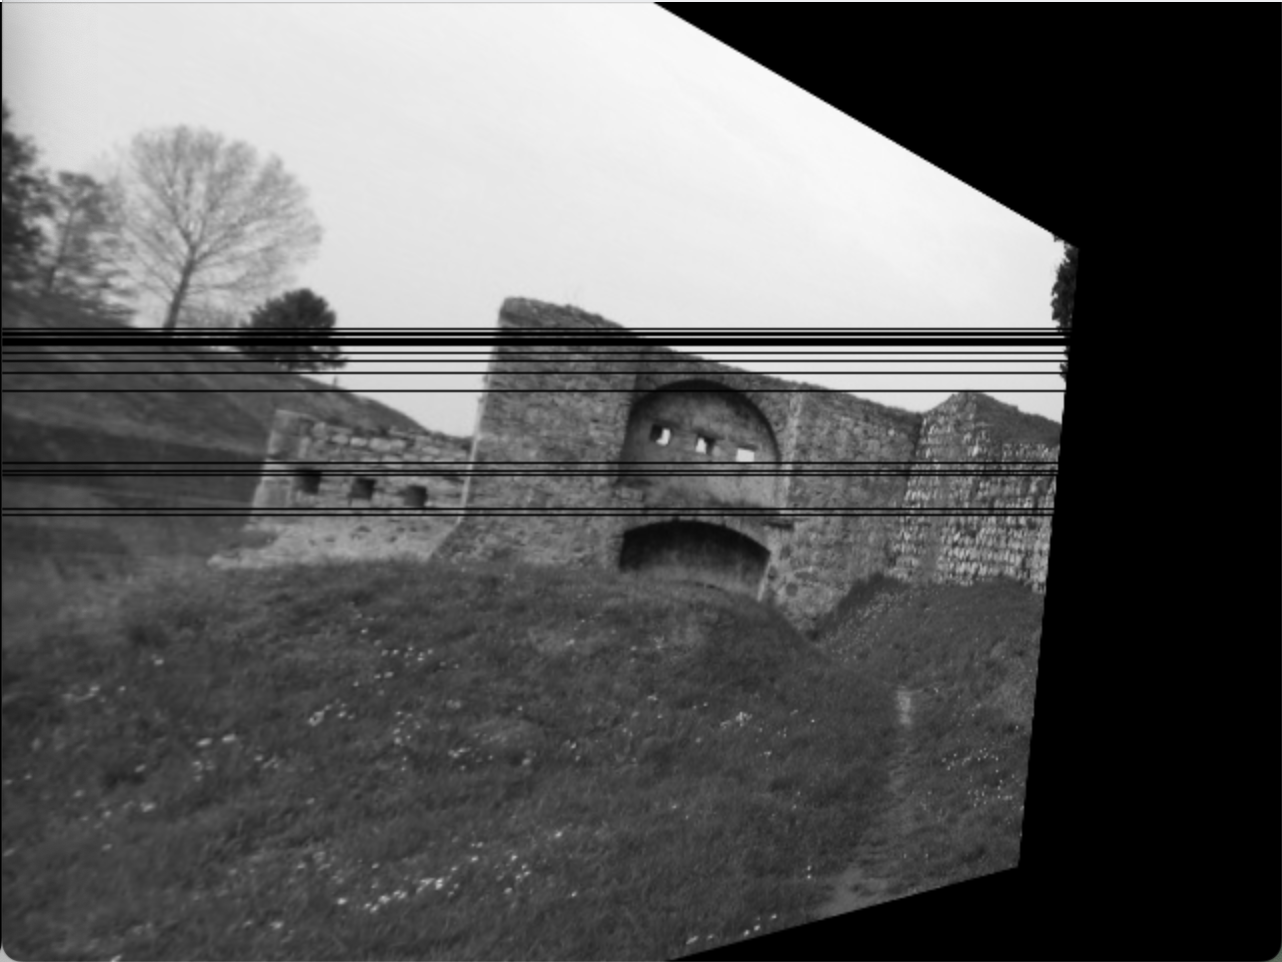
\includegraphics[width=\textwidth]{rect_left.png}}
    \centerline{Rectified Left Image}
    \end{minipage}
    \hfill
    \begin{minipage}[t]{0.32\textwidth}   
    \centerline{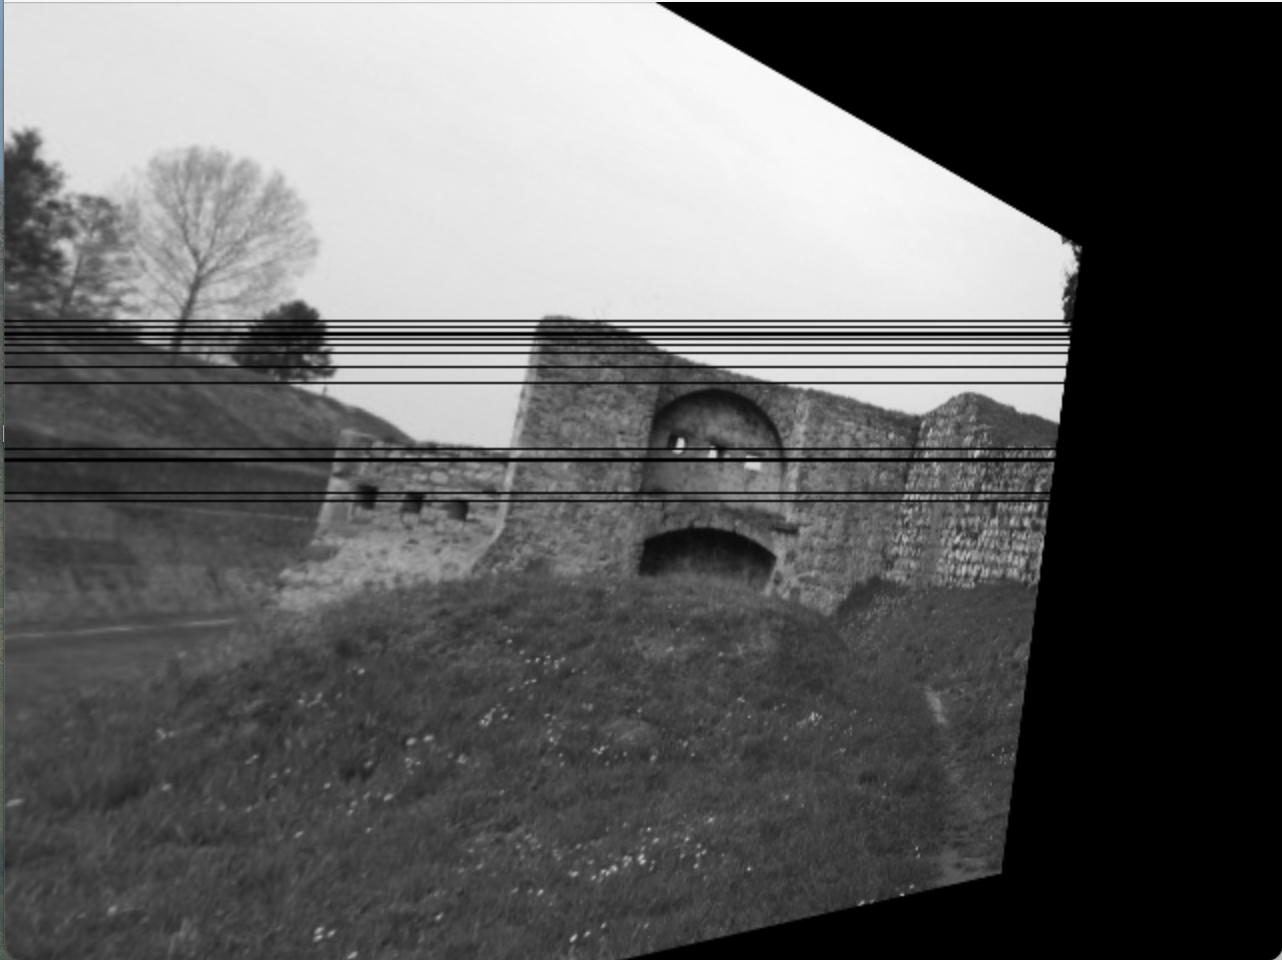
\includegraphics[width=\textwidth]{rect_right.png}}
    \centerline{Rectified Right Image}
    \end{minipage}
    \caption{Rectified Stereo pair of images}
    \label{fig:rectified stereo pair}
\end{figure}
Nevertheless, we can see that the rectification is not perfect in more difficult cases. In figure \ref{fig:comp} we can see that the the result of the ransac algorithm are far worth than the one obtained with LDMEDS (Least Median of Squares) algorithm. This is due to the fact that the LMEDS algorithm is more robust to outliers than the RANSAC algorithm.
\begin{figure}
    \centering
    \begin{minipage}[t]{0.5\textwidth}
    \centerline{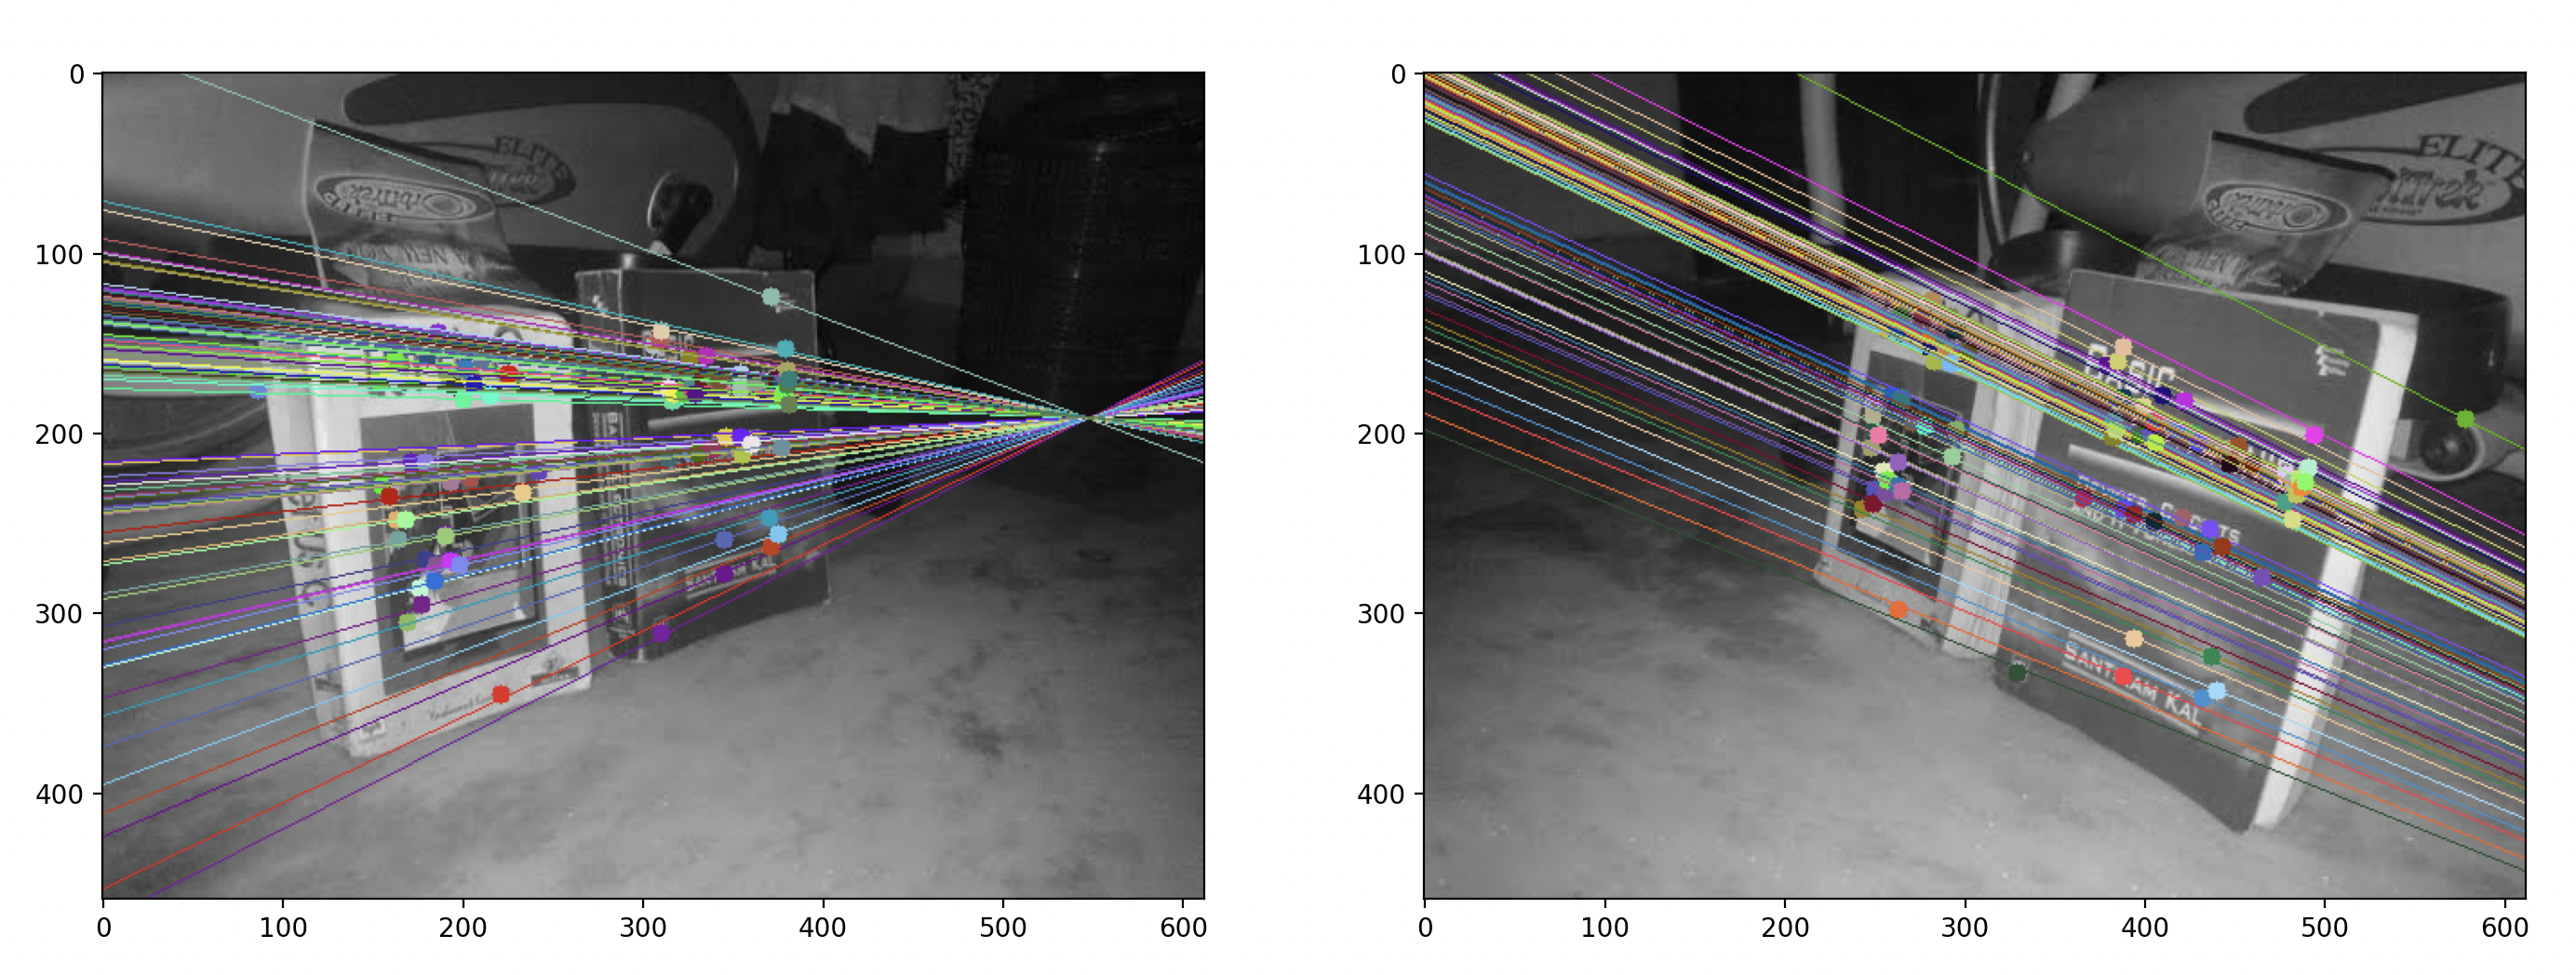
\includegraphics[width=\textwidth]{hard_ransac.png}}
    \centerline{Epipolar lines with RANSAC}
    \end{minipage}
    \hfill
    \begin{minipage}[t]{0.5\textwidth}   
    \centerline{\includegraphics[width=\textwidth]{hard_lmeds.png}}
    \centerline{Epipolar lines with LMEDS}
    \end{minipage}
    \caption{Comparaison with LMEDS algorithm (OpenCV implementation)}
    \label{fig:comp}
\end{figure}
\subsection{Disparity Map estimation}
\subsubsection{Test on middleburry image}

To test our disparity map algorithm we use a pair of images from the middleburry 2005 dataset (dolls). The left image of the pair, the estimated disparity map and the ground truth are given in figure \ref{fig:midlb}
\begin{figure}
    \centering
    \begin{minipage}[t]{0.4\textwidth}
    \centerline{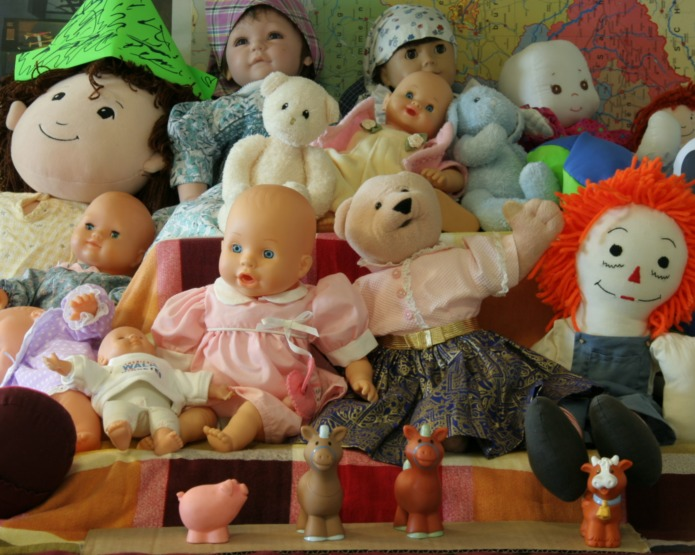
\includegraphics[width=\textwidth]{midb1.jpg}}
    \centerline{Left image of the stereo pair}
    \end{minipage}
    \hfill
    \begin{minipage}[t]{0.23\textwidth}   
    \centerline{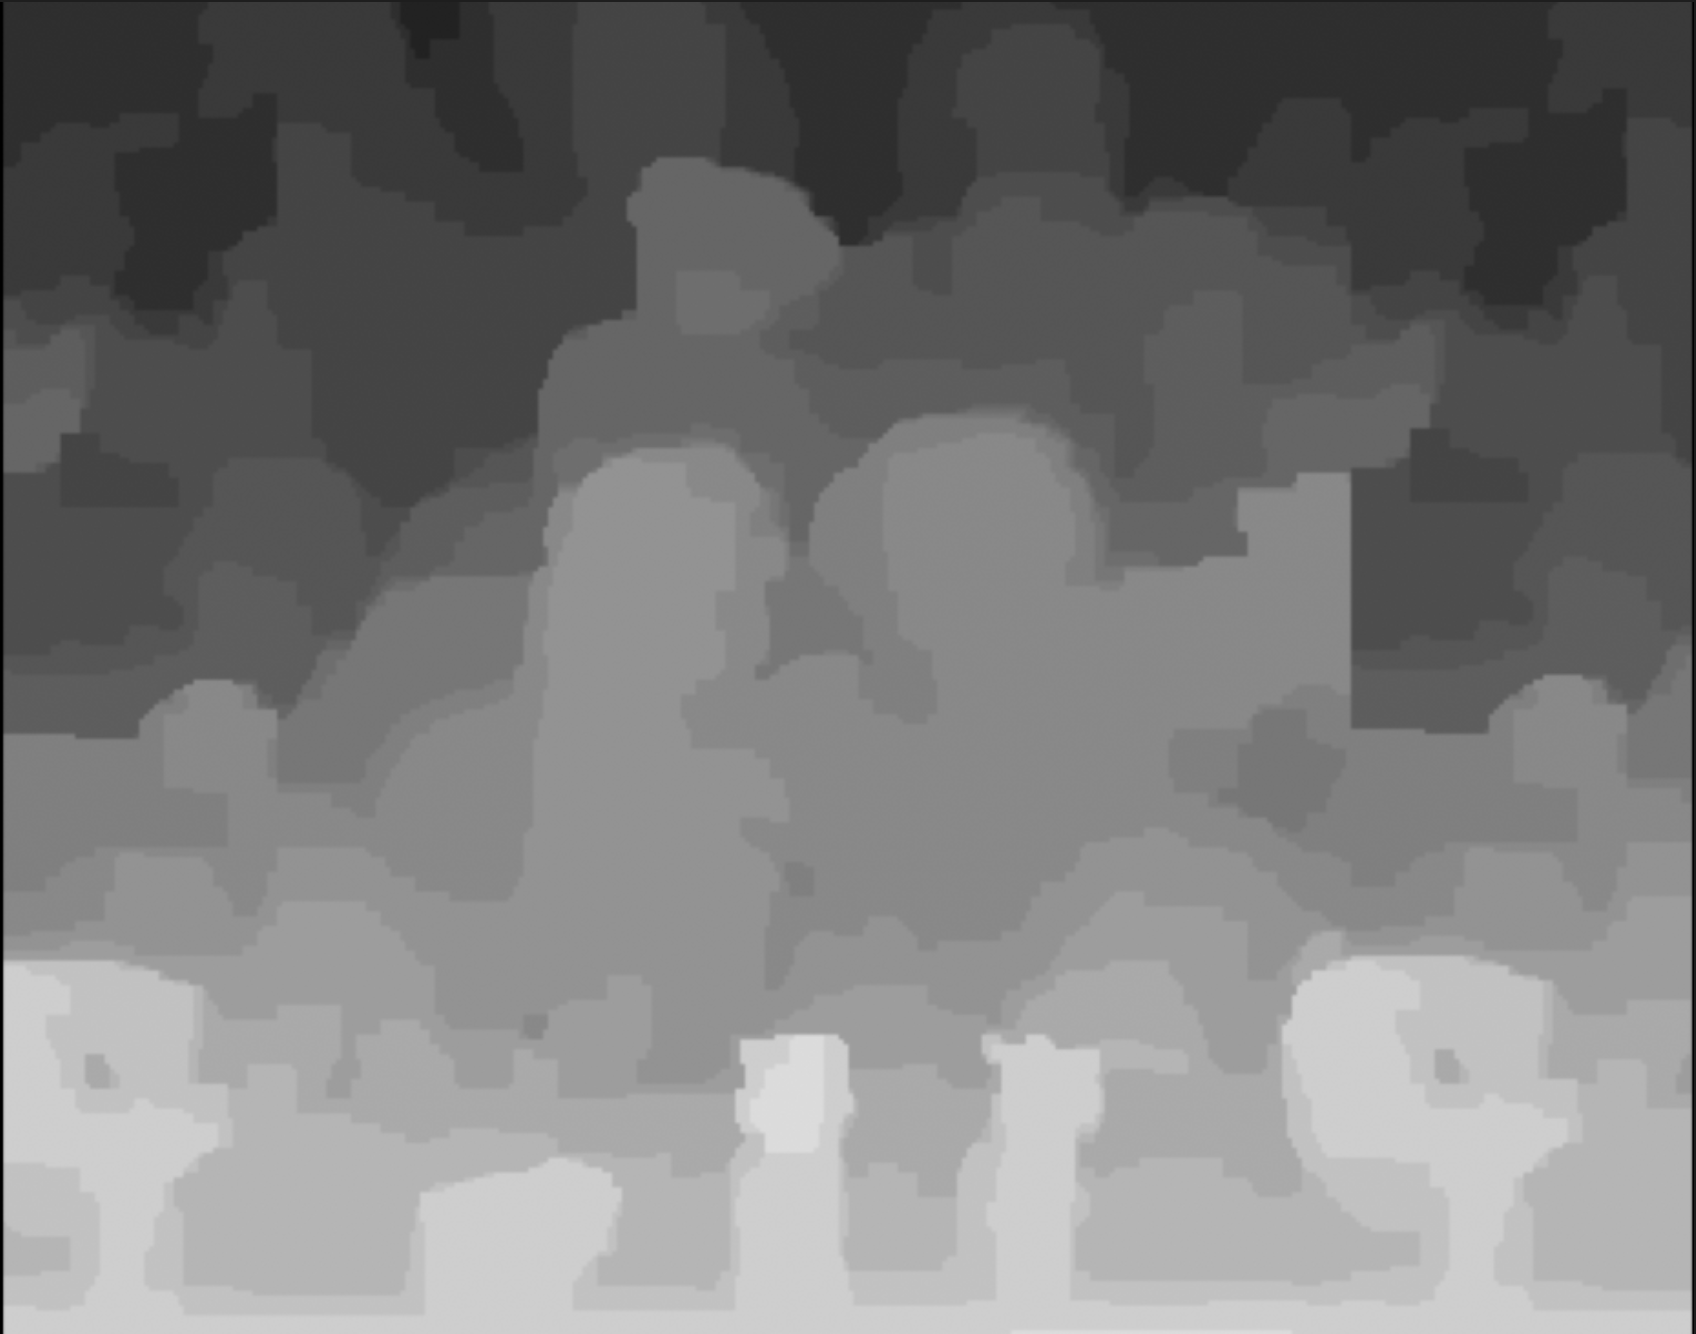
\includegraphics[width=\textwidth]{output_midlb.png}}
    \centerline{Estiamted disparity map}
    \end{minipage}
    \begin{minipage}[t]{0.23\textwidth}   
        \centerline{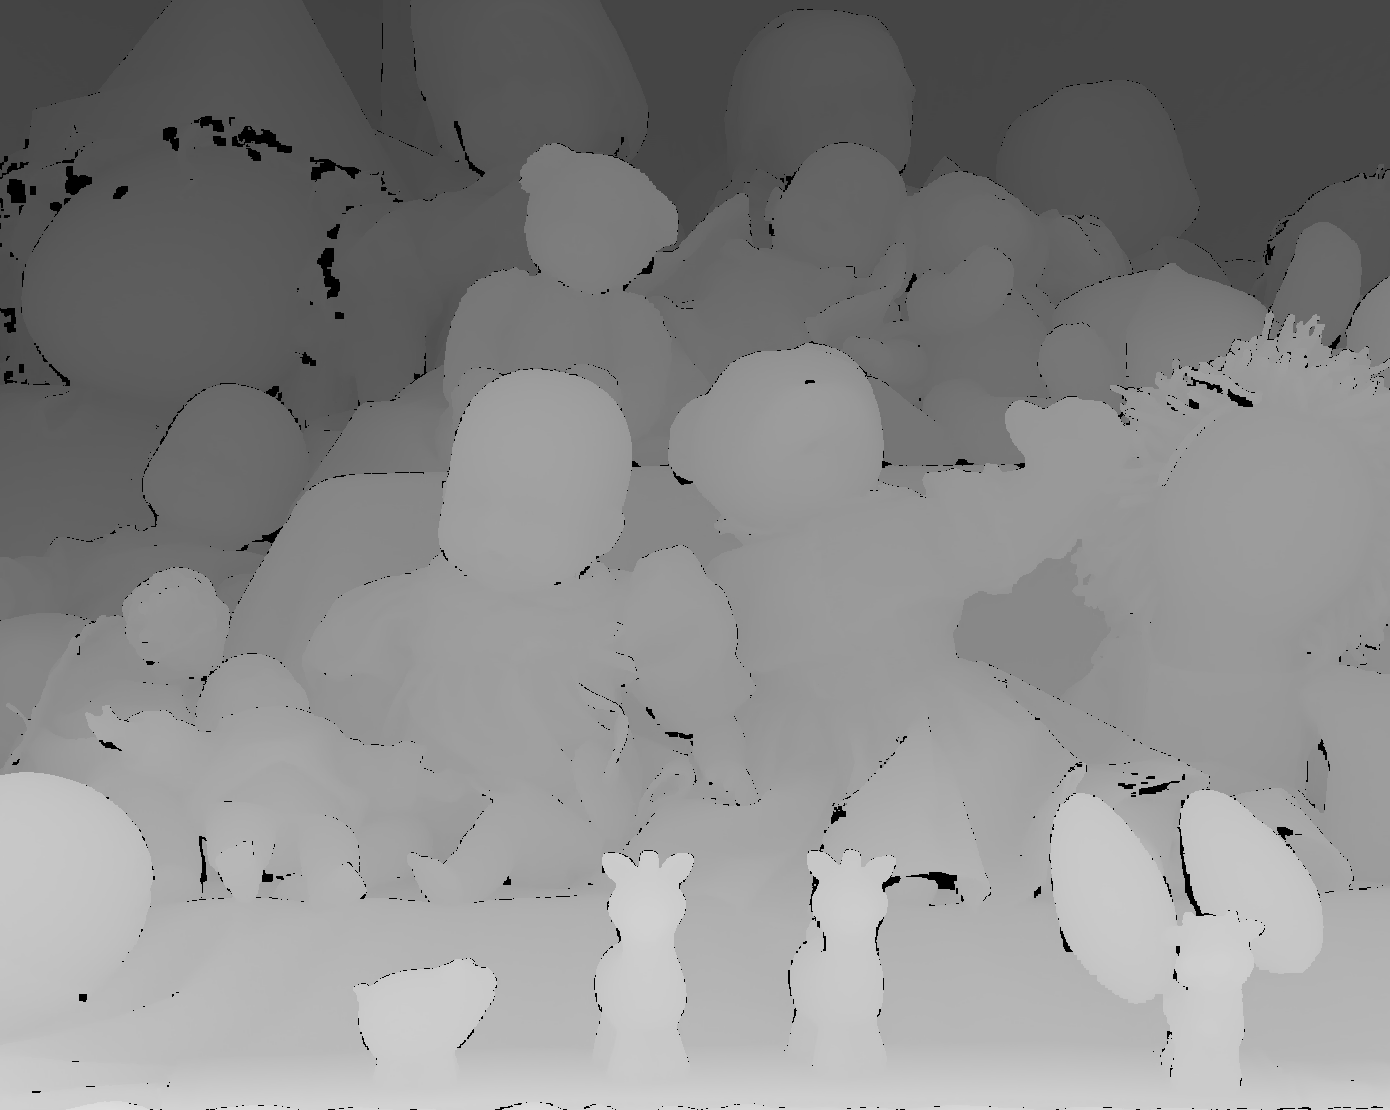
\includegraphics[width=\textwidth]{gt_midlb.png}}
        \centerline{Ground truth disparity map}
        \end{minipage}
    \caption{Disparity map estimation on middleburry dataset}
    \label{fig:midlb}
\end{figure}

While the result is not perfect especially in some part of the image (look at the clown on the left on the image). We believe that the result of the disparity map estimation are satisfying.

\subsubsection{Extra terrestrial data}
Finally we test our algorithm for the presented task "reconstruction of terrain topography". While AMES Stereo pipeline was more difficult to use than previously anticipated (especially because of the ISIS package used to process most of the images and that we did not manage to install on our machine); we nevertheless managed to run the pipeline on a simple example given along with the output of the pipeline in figure \ref{fig:moon}. 
\begin{figure}
    \centering
    \begin{minipage}[t]{0.22\textwidth}
    \centerline{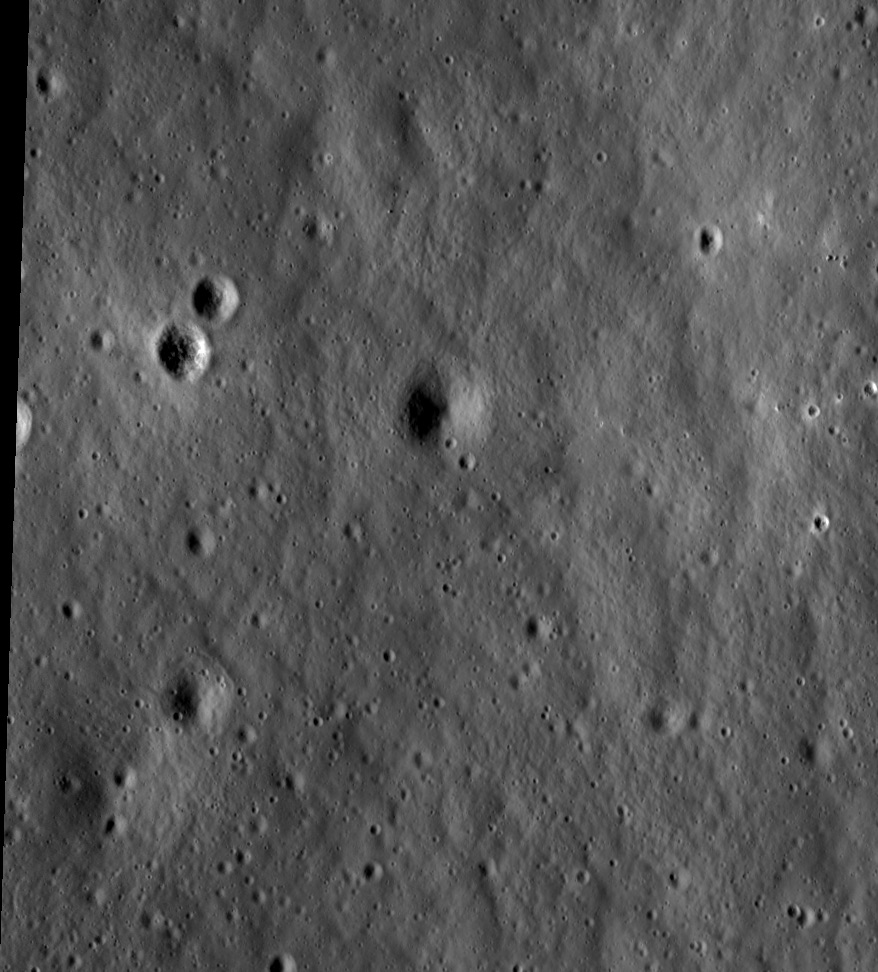
\includegraphics[width=\textwidth]{run-L.jpeg}}
    \centerline{Left image}
    \end{minipage}
    \hfill
    \begin{minipage}[t]{0.23\textwidth}   
    \centerline{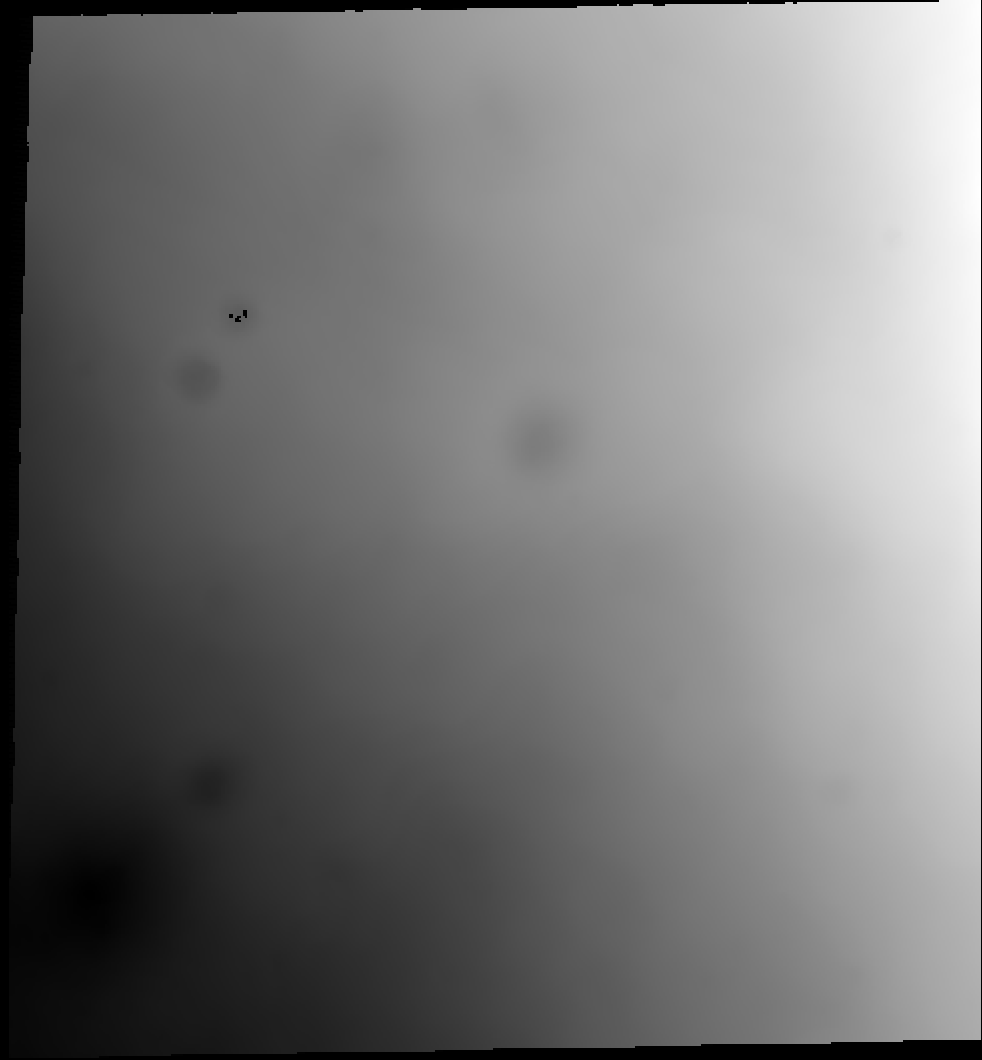
\includegraphics[width=\textwidth]{ames_out.png}}
    \centerline{Disparity map (AMES pipeline)}
    \end{minipage}
    \caption{Disparity map estimation on extra terrestrial data (AMES pipeline)}
    \label{fig:moon}
\end{figure}
We then run our pipeline. First we compute the epipolar line and we can see on figure \ref{fig:moon_epi} that there is no need for rectification as the lines are parallel.
\begin{figure}
    \centering
    \includegraphics[width=0.5\textwidth]{epi_moon.png}
    \caption{Epipolar lines on extra terrestrial data}
    \label{fig:moon_epi}
\end{figure}
Finally we run the algorithm and get the result given on figure \ref{fig:moon_out}. This is not a final result as and further postprocessing is needed (and done in AMES) for comparaison we give the un-postprocessed disparity map outputed by ames. On this noisy image we can see the small hills at the center of the image but there is also a lot of noise at the bottom and top of the image, the goal of the rest of the pipeline is to remove this noise but will not consider the rest of the pipeline in this project.
\begin{figure}
    \centering
    \begin{minipage}[t]{0.22\textwidth}
    \centerline{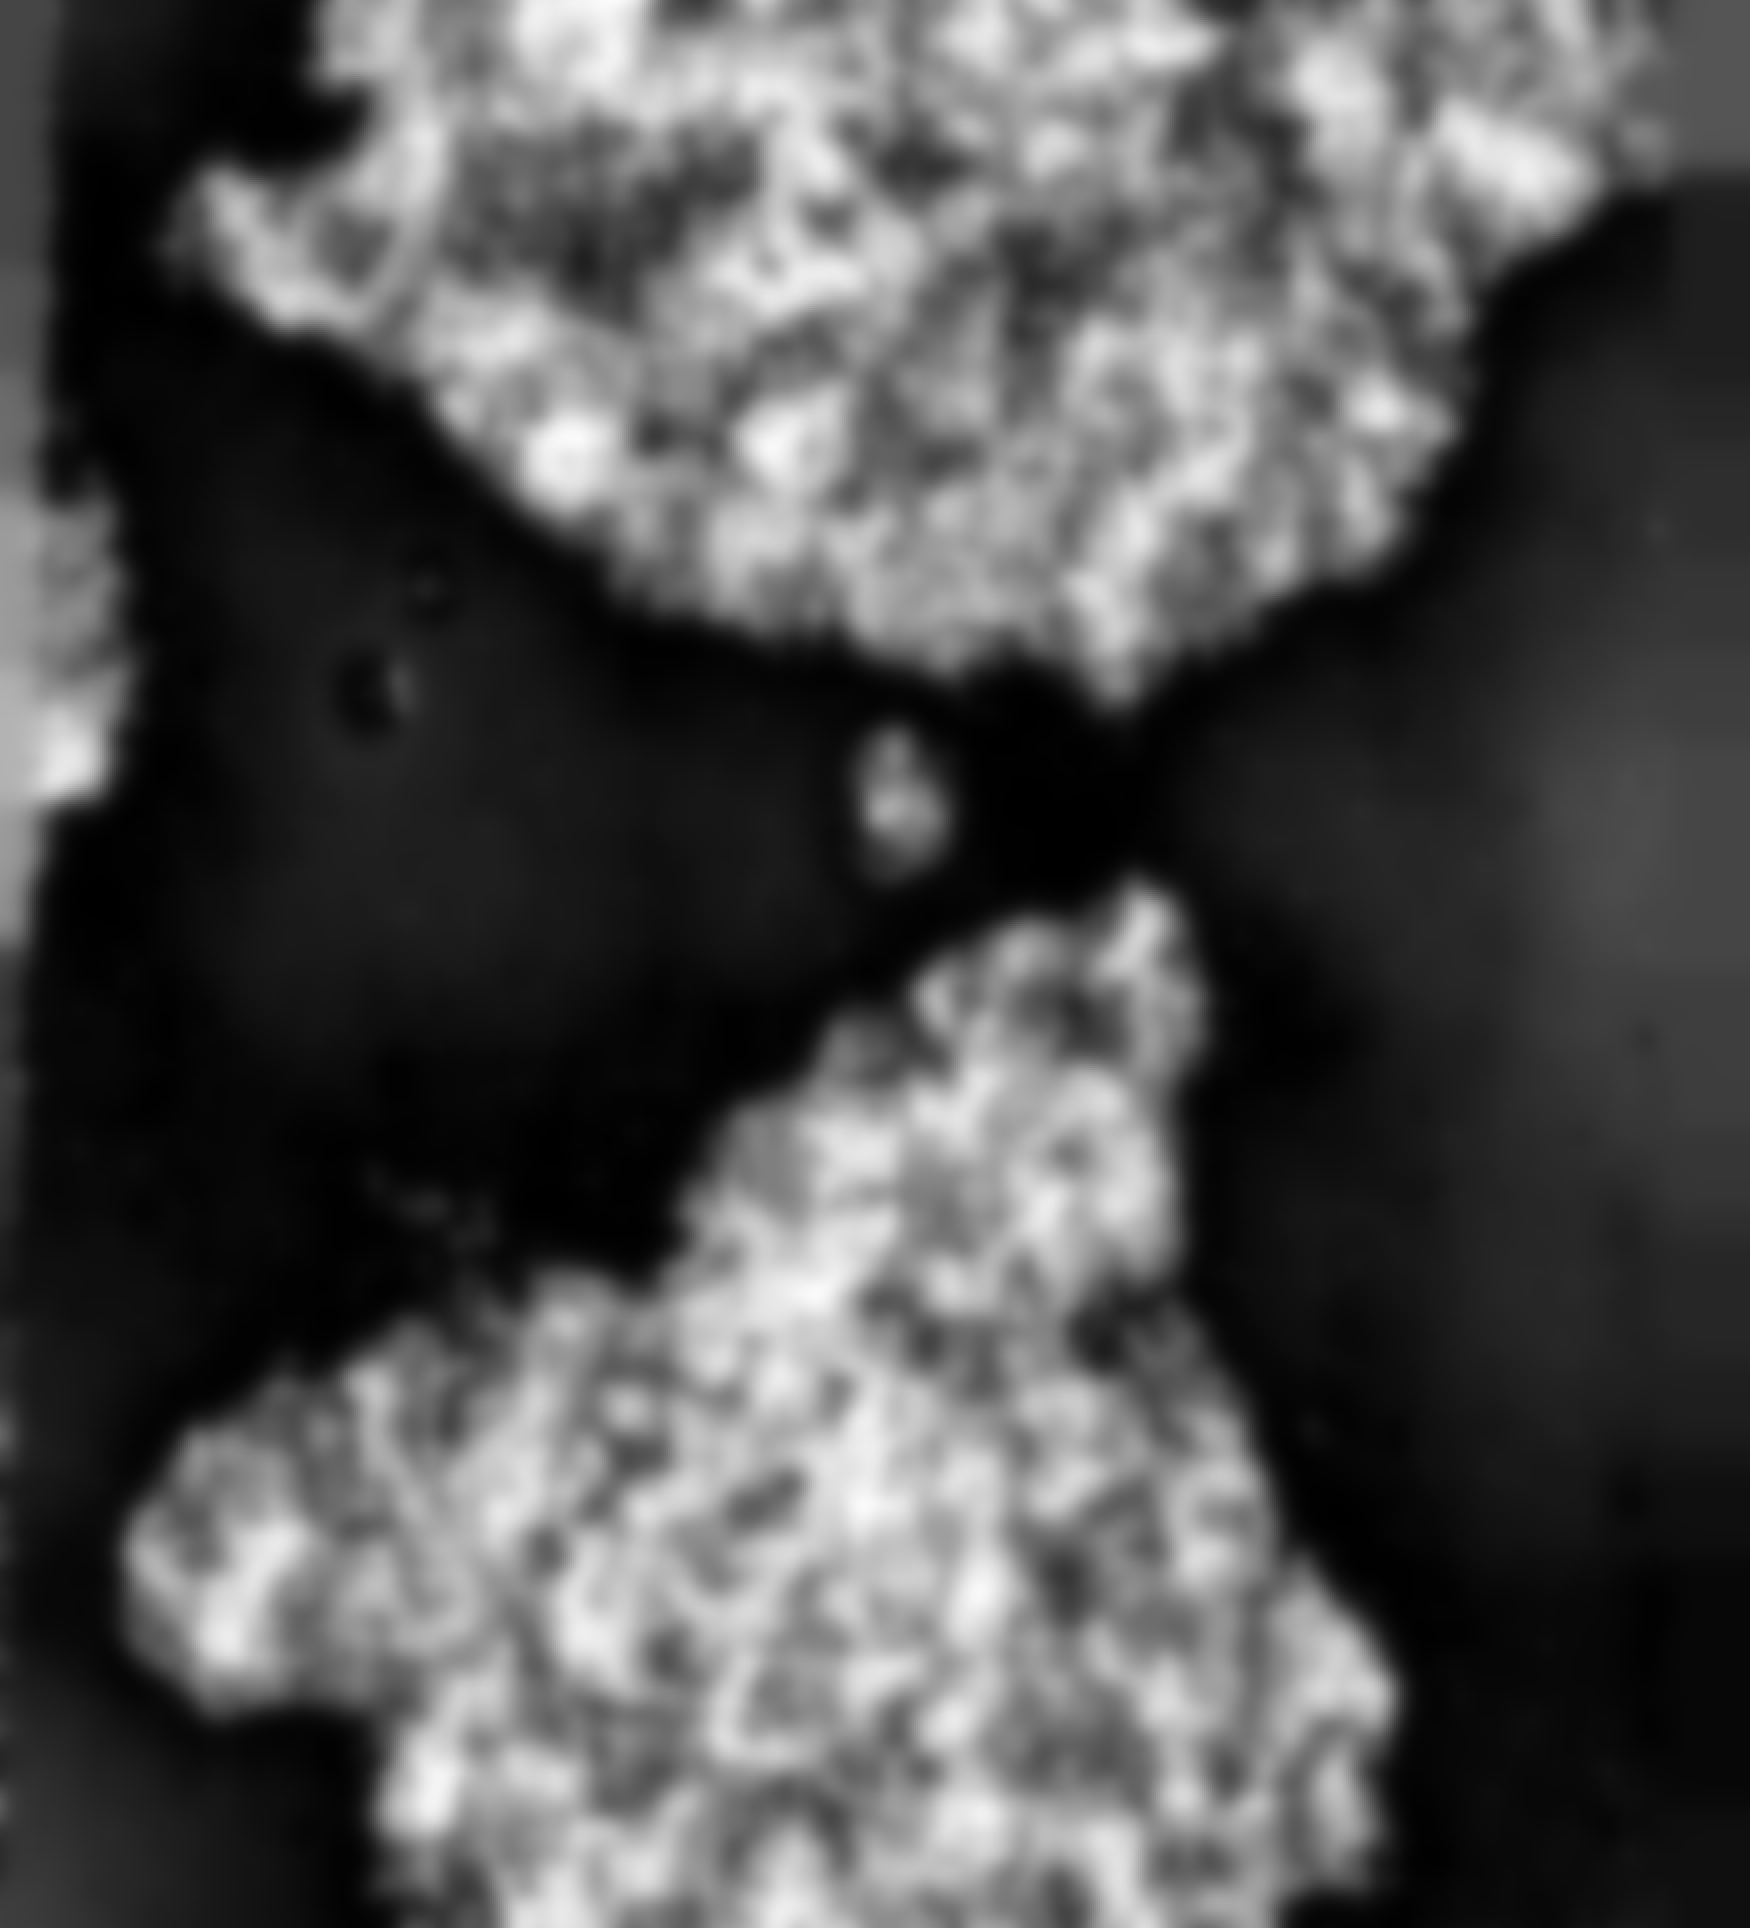
\includegraphics[width=\textwidth]{out_moon.png}}
    \centerline{our pipeline}
    \end{minipage}
    \hfill
    \begin{minipage}[t]{0.23\textwidth}   
    \centerline{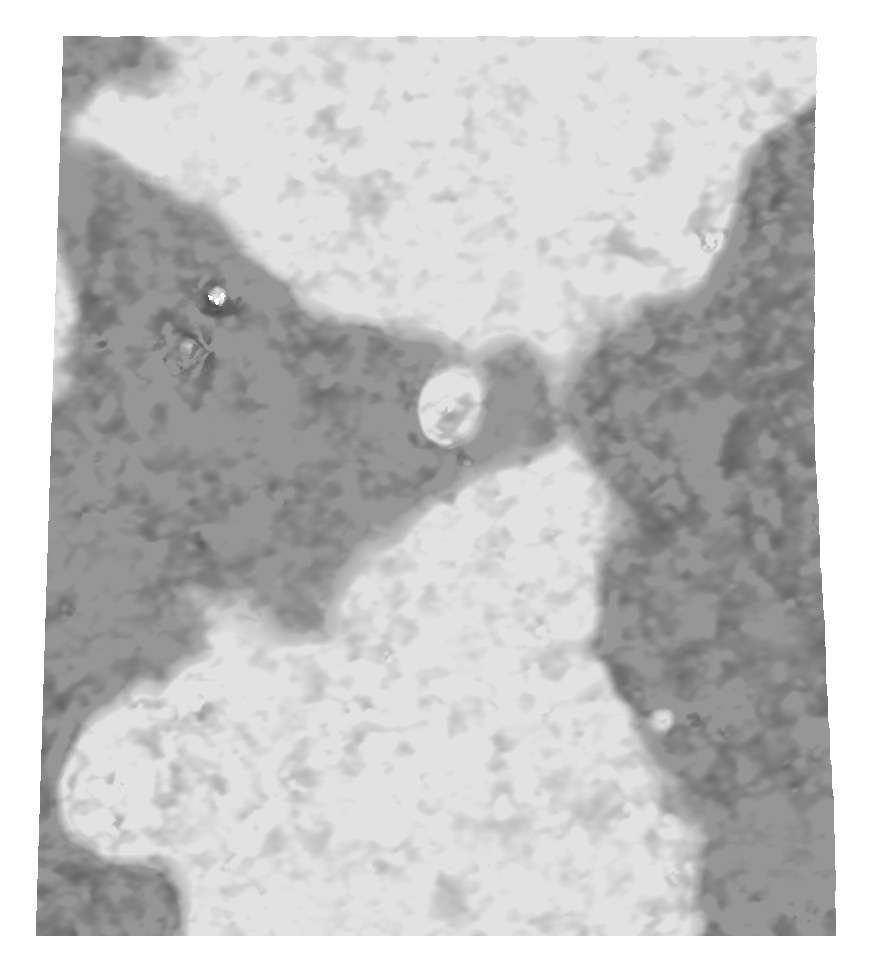
\includegraphics[width=\textwidth]{out_moon_gt.jpeg}}
    \centerline{AMES pipeline}
    \end{minipage}
    \caption{Noisy disparity map estimation on extra terrestrial data (AMES pipeline)}
    \label{fig:moon_out}
\end{figure}
\section{Conclusion}
In this project, we have implemented a disparity map estimation algorithm for stereo vision. We have tested our algorithm on various datasets, including the Middlebury dataset and extra terrestrial data. 

Overall, our algorithm has shown promising results in estimating the disparity map. However, there are still areas for improvement, especially in handling challenging cases with occlusions (which we didn't test in our project but is a know problem in disparity map estimation) and noise. 

Future work could focus on refining the algorithm to improve its accuracy and robustness, especially implementing LMEDS for the epipolar rectification and potentialy invest various deep learning methods that are the deep equivalent of the methods used in the project namely \cite{lindebergScaleInvariantFeature2012} \cite{fischlerRandomSampleConsensus1981} \cite{hirschmullerAccurateEfficientStereo2005a}. Additionally, further post-processing techniques could be explored to enhance the quality of the disparity maps. 

Despite the limitations, this project has provided valuable insights into stereo vision and its applications in depth perception. It has also highlighted the importance of choosing appropriate algorithms and datasets for evaluation. 

In conclusion, stereo vision and disparity map estimation are important areas of research with numerous practical applications. By continuing to refine and optimize these algorithms, we can unlock their full potential in various fields such as robotics, autonomous vehicles, and augmented reality.


\newpage
\printbibliography
\end{document}
